\documentclass[10pt]{article}
\usepackage{ucs}
\usepackage[a4paper, total={7in, 10in}]{geometry}
\usepackage[cp1251]{inputenc}
\usepackage{graphicx}
\title{CIA: Assignment Web Servers}
\date{5 October 2016}
\author{Ali Abdulmadzhidov}

\begin{document}
\renewcommand*\rmdefault{cmss}
\maketitle
1. Because of growth of Google maybe. They start using their own solution. Also we got new webservers like nginx that got their part of a cake
\section{Installation}
\begin{enumerate}
    \item Downloading sources
    \begin{verbatim}wget http://apache-mirror.rbc.ru/pub/apache//httpd/httpd-2.4.23.tar.gz\end{verbatim}
    \item Downloading signature
    \begin{verbatim}wget https://www.apache.org/dist/httpd/httpd-2.4.23.tar.gz.asc\end{verbatim}
    \item Checking signature.. Got error that public key not found
    \begin{verbatim}gpg --verify httpd-2.4.23.tar.gz.asc\end{verbatim}
    \item Getting key from remote by id
    \begin{verbatim}gpg --keyserver pool.sks-keyservers.net --recv-keys 0x791485A8 \end{verbatim}
    \item Second successfull try to check signature
    \begin{verbatim}
        gpg --verify httpd-2.4.23.tar.gz.asc

        gpg: Signature made Thu 30 Jun 2016 20:15:21 MSK using RSA key ID 791485A8
        gpg: Good signature from "Jim Jagielski (Release Signing Key) <jim@apache.org>"
        gpg:                 or "Jim Jagielski <jim@jimjag.com>"
        gpg:                 or "Jim Jagielski <jim@jaguNET.com>"
        gpg:                 or "Jim Jagielski <jimjag@gmail.com>"
        gpg: WARNING: This key is not certified with a trusted signature!
        gpg:          There is no indication that the signature belongs to the owner.
        Primary key fingerprint: A93D 62EC C3C8 EA12 DB22  0EC9 34EA 76E6 7914 85A8
    \end{verbatim}
    \item Extracting archive with sources
    \begin{verbatim}
        tar -xzvf httpd-2.4.23.tar.gz
    \end{verbatim}
    \item After reading README and ./configuration --help trying to configure with ssl. Got error that apr and apr-util are missing
    \begin{verbatim}
        ./configure --enable-ssl=shared
    \end{verbatim}
    \item Downloading them, their signatures, checking them and extracting them to srclib folder
    \begin{verbatim}
        wget http://apache-mirror.rbc.ru/pub/apache//apr/apr-1.5.2.tar.gz
        wget http://apache-mirror.rbc.ru/pub/apache//apr/apr-util-1.5.4.tar.gz
        ...
        mv apr-1.5.2 httpd-2.4.23/srclib/apr
        mv apr-util-1.5.4 httpd-2.4.23/srclib/apr-util
    \end{verbatim}
    \item Second try to configure, now with --with-included-apr
    \begin{verbatim}
        ./configure --enable-ssl=shared --with-included-apr
    \end{verbatim}
    \item Make and make install
    \item Making symling for apachectl to /usr/bin
    \begin{verbatim}ln -s /usr/local/apachectl /usr/bin \end{verbatim}
    \item Writing init.d script to make apache start on boot
    \begin{verbatim}
        > nano /etc/init.d/apache2
        #!/bin/bash
        #
        # apache2        Startup script for the Apache HTTP Server
        #
        # description: Apache is a World Wide Web server.  It is used to serve \
        #              HTML files and CGI.

        /usr/local/apache2/bin/apachectl $@

        > chmod 755 /etc/init.d/apache2
        > update-rc.d apache2 defaults
    \end{verbatim}
    \item Checking our webserver
    \begin{verbatim}
        > service apache2 restart
        > curl 127.0.0.1
        It's working
    \end{verbatim}
    \item Going to look and update config file
    \begin{verbatim}
        > nano /usr/local/a/conf/htt
        Listen 8080 # Change port
        DocumentRoot "/var/www"  # Where out site'll reside
        ServerName st9.os3.su #Our servername
        ServerAdmin ali@mail.st9.os3.su
    \end{verbatim}
    \item Going to look and update config file
    \begin{verbatim}
        > nano /usr/local/a/conf/htt
        ...
        Listen 8080 # Change port
        DocumentRoot "/var/www"  # Where out site'll reside
        ServerName st9.os3.su #Our servername
        ServerAdmin ali@mail.st9.os3.su
        ...
    \end{verbatim}
\end{enumerate}

2. Maybe cause it still used. For example Red Hat 5 and 6 use Apache 2.2.3 and 2.2.15, with necessary backported patches applied. \cite{redhat}

\section{Virtual hosts}
\begin{enumerate}
\item Firstly check that we have two subdomains from our neighboors with A RR's to our address
\begin{verbatim}
> host st9.st10.os3.su
st9.st10.os3.su has address 188.130.155.42
> host st9.st8.os3.su
st9.st8.os3.su has address 188.130.155.42
\end{verbatim}
\item Creating two folders to content subdomains files.
\begin{verbatim}
    > mkdir /var/www/st10
    > echo `st10' > index.html
    > mkdir /var/www/st8
    > echo `st8' > index.html
    > chmod -R 755 /var/www/*
\end{verbatim}
\item Going to webserver's config to set up our virtual domains. I chose to configure my server with 3 virtual hosts, cause it makes easy to divide them and implement https
\begin{verbatim}
    <VirtualHost st9.os3.su:8080>
        DocumentRoot "/var/www"
        ServerName st9.st10.os3.su
    </VirtualHost>
    <VirtualHost st9.st10.os3.su:8080>
        DocumentRoot "/var/www/st10"
        ServerName st9.st10.os3.su
    </VirtualHost>
    <VirtualHost st9.st8.os3.su:8080>
        DocumentRoot "/var/www/st8"
        ServerName st9.st8.os3.su
    </VirtualHost>
\end{verbatim}

\item Checking with curl
\begin{verbatim}
> curl -v st9.st10.os3.su:8080
* Rebuilt URL to: st9.st10.os3.su:8080/
*   Trying 188.130.155.42...
* Connected to st9.st10.os3.su (188.130.155.42) port 8080 (#0)
> GET / HTTP/1.1   #Says that we make get request to host's root by HTTP1.1 
> Host: st9.st10.os3.su:8080 # The domain name of the server and port. 
We don't need write port if we request to default 80. This field is required by HTTP1.1
> User-Agent: curl/7.47.0 # Useragent shows from which app request was maded
> Accept: */* # Content types that are acceptable for the response. 
>
< HTTP/1.1 200 OK # Shows response protocol and status of response. It can be 404 Not Found, 500 Internal server error, 403 Forbiden or if all is fine 200 OK like here
< Date: Thu, 06 Oct 2016 17:34:05 GMT # Time when response was created
< Server: Apache/2.4.23 (Unix) # Server and version
< Last-Modified: Thu, 06 Oct 2016 08:32:49 GMT # The last modified time for the server
< ETag: "5b99-53e2e238f697c" # Idintifier of response, needed to make caching more efficient
< Accept-Ranges: bytes # Defines what  content parts server supports
< Content-Length: 23449 # Length of response in bytes
< Content-Type: text/html # Type of response
<

Second host

> curl -v st9.st8.os3.su:8080
* Rebuilt URL to: st9.st8.os3.su:8080/
*   Trying 188.130.155.42...
* Connected to st9.st8.os3.su (188.130.155.42) port 8080 (#0)
> GET / HTTP/1.1
> Host: st9.st8.os3.su:8080
> User-Agent: curl/7.47.0
> Accept: */*
>
< HTTP/1.1 200 OK
< Date: Thu, 06 Oct 2016 17:48:39 GMT
< Server: Apache/2.4.23 (Unix)
< Last-Modified: Thu, 06 Oct 2016 08:28:35 GMT
< ETag: "1d2e-53e2e1466871c"
< Accept-Ranges: bytes
< Content-Length: 7470
< Content-Type: text/html
<
\end{verbatim}
\end{enumerate}

\section{Encryption}
\begin{enumerate}
    \item Go to config
    \begin{verbatim}
        Listen 443 # Change 8080 to 443 cause https works on that port
        ...
        <VirtualHost st9.os3.su:443>
            DocumentRoot "/var/www"
            ServerName st9.os3.su
            SSLEngine on #turns on SSL
            <Directory>
            SSLRequireSSL # Let's load this dir only through secure connection
            </Directory>
            SSLOptions +StrictRequire 
            #Locks access when SSLRequireSSL decided that access should be denied.
            
            SSLProtocol All -TLSv1 -SSLv2 -SSLv3 -TLSv1.1
            # Turns off all unsecure versions of SSL/TLS. Left only TLSv1.2
            
            SSLCipherSuite EECDH+AESGCM:EDH+AESGCM:AES256+EECDH:ECDHE-RSA-AES128-SHA
            :DHE-RSA-AES128-GCM-SHA256:AES256+EDH:ECDHE-RSA-AES256-GCM-SHA384
            :ECDHE-RSA-AES128-GCM-SHA256:DHE-RSA-AES256-GCM-SHA384:ECDHE-RSA-AES256-SHA384
            :ECDHE-RSA-AES128-SHA256:ECDHE-RSA-AES256-SHA:DHE-RSA-AES256-SHA256
            :DHE-RSA-AES128-SHA256:DHE-RSA-AES256-SHA:DHE-RSA-AES128-SHA
            :ECDHE-RSA-DES-CBC3-SHA:EDH-RSA-DES-CBC3-SHA:AES256-GCM-SHA384:AES128-GCM-SHA256
            :AES256-SHA256:AES128-SHA256:AES256-SHA:AES128-SHA:DES-CBC3-SHA:HIGH:!aNULL
            :!eNULL:!EXPORT:!DES:!MD5:!PSK:!RC4
            # Cipher suites that i decided to left for different situations. I'll describe this below
            
            SSLCompression off 
            # Turn compression off, cause turning on lefts way to CRIME attack
            
            SSLCertificateFile /usr/local/apache2/conf/ssl.crt/server.crt 
            # st crt that Azat gave to us
            
            SSLCertificateKeyFile /usr/local/apache2/conf/ssl.key/server.key 
            # key from Azat
            
            SSLCertificateChainFile /usr/local/apache2/conf/ssl.crt/root.crt 
            # root for security chain. Got from Azat
        </VirtualHost>
        ...
        SSLRandomSeed startup file:/dev/urandom 1024 
        SSLRandomSeed connect file:/dev/urandom 1024
        #settings for generation random values for OpenSSL
        Mutex file:/usr/local/apache2/logs/ssl_mutex #set's mutex file for ssl
        SSLSessionCache shmcb:/usr/local/apache2/logs/ssl_cache_shm # SSLCache storage
        SSLSessionCacheTimeout 600 #timeout in seconds
    \end{verbatim}
    \item Cipher choose 
        ECDHE+AESGCM first, cause this are TLSv2 and no attacks are nown on them
        AES 128 is preffered on 256 cause it's faster and gains needed secruity level
        3DES is added for back compbility
        RC4 is too weak and removed
        aNULL contains way to make MITM attacks
        EXPORT are weak ciphers
        DES, MD5 and SSLv2 contains deprecated ciphers
    \item We got certificate from Azat, but we can create one 
    \begin{verbatim}
        openssl req -new -x509 -days 30 -keyout /usr/local/apache2/conf/ssl.key/server.key -out /usr/local/apache2/conf/ssl.crt/server.crt -subj '/CN=Test-Only Certificate'
    \end{verbatim}
    But this cert wouldn't be verified by browser. For that we should go to specialized services and get signed certificate. For example https://letsencrypt.org/
    \item We got certificate from Azat, but we can create one 
    \begin{verbatim}
        openssl req -new -x509 -days 30 -keyout /usr/local/apache2/conf/ssl.key/server.key -out /usr/local/apache2/conf/ssl.crt/server.crt -subj '/CN=Test-Only Certificate'
    \end{verbatim}
    But this cert wouldn't be verified by browser. For that we should go to specialized services and get signed certificate. For example https://letsencrypt.org/
    \item Checking ssl with openssl and curl
    \begin{verbatim}
        openssl s_client -connect st9.os3.su:443
        CONNECTED(00000003)
        depth=2 C = IL, O = StartCom Ltd., OU = Secure Digital Certificate Signing, CN = StartCom Certification Authority
        verify return:1
        depth=1 C = IL, O = StartCom Ltd., OU = StartCom Certification Authority, CN = StartCom Class 4 EV Server CA
        verify return:1
        depth=0 jurisdictionC = RU, jurisdictionST = Tatarstan, jurisdictionL = Innopolis, businessCategory = Non-Commercial Entity, serialNumber = 1121600006142, C = RU, ST = Tatarstan, L = Innopolis, postalCode = 420500, street = "Universitetskaya Str, 1", O = Innopolis University, CN = st.os3.su
        verify return:1
        ---
        Certificate chain
         0 s:/jurisdictionC=RU/jurisdictionST=Tatarstan/jurisdictionL=Innopolis/businessCategory=Non-Commercial Entity/serialNumber=1121600006142/C=RU/ST=Tatarstan/L=Innopolis/postalCode=420500/street=Universitetskaya Str, 1/O=Innopolis University/CN=st.os3.su
           i:/C=IL/O=StartCom Ltd./OU=StartCom Certification Authority/CN=StartCom Class 4 EV Server CA
         1 s:/C=IL/O=StartCom Ltd./OU=StartCom Certification Authority/CN=StartCom Class 4 EV Server CA
           i:/C=IL/O=StartCom Ltd./OU=Secure Digital Certificate Signing/CN=StartCom Certification Authority
        ---
        Server certificate
        -----BEGIN CERTIFICATE-----
        MIII8DCCB9igAwIBAgIQSoTS6IdBhvQ++UOPpZaJVTANBgkqhkiG9w0BAQsFADB4
        MQswCQYDVQQGEwJJTDEWMBQGA1UEChMNU3RhcnRDb20gTHRkLjEpMCcGA1UECxMg
        U3RhcnRDb20gQ2VydGlmaWNhdGlvbiBBdXRob3JpdHkxJjAkBgNVBAMTHVN0YXJ0
        Q29tIENsYXNzIDQgRVYgU2VydmVyIENBMB4XDTE2MDkzMDA5NTQzM1oXDTE4MDkz
        MDA5NTQzM1owggEgMRMwEQYLKwYBBAGCNzwCAQMTAlJVMRowGAYLKwYBBAGCNzwC
        AQIMCVRhdGFyc3RhbjEaMBgGCysGAQQBgjc8AgEBDAlJbm5vcG9saXMxHjAcBgNV
        BA8MFU5vbi1Db21tZXJjaWFsIEVudGl0eTEWMBQGA1UEBRMNMTEyMTYwMDAwNjE0
        MjELMAkGA1UEBhMCUlUxEjAQBgNVBAgMCVRhdGFyc3RhbjESMBAGA1UEBwwJSW5u
        b3BvbGlzMQ8wDQYDVQQRDAY0MjA1MDAxIDAeBgNVBAkMF1VuaXZlcnNpdGV0c2th
        eWEgU3RyLCAxMR0wGwYDVQQKDBRJbm5vcG9saXMgVW5pdmVyc2l0eTESMBAGA1UE
        AwwJc3Qub3MzLnN1MIIBIjANBgkqhkiG9w0BAQEFAAOCAQ8AMIIBCgKCAQEAxKkL
        QYi43fSyMHkDuO1L4qlebWIGZBZTQL0GThSjKyeX71qfAsj9ezeYTMF8C1uLYhlx
        tuJRYnZV+bED6LIX6bWuHmd3GqY6Otv/ATAF/kyowB9esybCLEtzg5Hwl5cfjjvd
        oOWzAldZtjdeUebiC/2nSH/HZdaSzIoevPEf2/wRybhPfQoHUnChM2KiSyCD9HOw
        MkWKoiIhsf5hayJzXIDv4qzk0wP8Hkwk4gldROnrhf3sQA65zxxmtceAMw2Zrw4t
        DmK6Ls5/nRNLOc/GwkzSUQV88Hf45ZDpv+i4vJv6jdKIHCG8IKfrQkSya3XtvuXa
        wyQiYRqWmXRybo28RQIDAQABo4IEyjCCBMYwDgYDVR0PAQH/BAQDAgWgMB0GA1Ud
        JQQWMBQGCCsGAQUFBwMCBggrBgEFBQcDATAJBgNVHRMEAjAAMB0GA1UdDgQWBBRH
        GyeovHEx/OKAjzCrgR+jQFK7yjAfBgNVHSMEGDAWgBQO2A3SZh2rcraJZUtkPX4Y
        J9SM3jBvBggrBgEFBQcBAQRjMGEwJAYIKwYBBQUHMAGGGGh0dHA6Ly9vY3NwLnN0
        YXJ0c3NsLmNvbTA5BggrBgEFBQcwAoYtaHR0cDovL2FpYS5zdGFydHNzbC5jb20v
        Y2VydHMvc2NhLnNlcnZlcjQuY3J0MDgGA1UdHwQxMC8wLaAroCmGJ2h0dHA6Ly9j
        cmwuc3RhcnRzc2wuY29tL3NjYS1zZXJ2ZXI0LmNybDCB0AYDVR0RBIHIMIHFgglz
        dC5vczMuc3WCCnN0MS5vczMuc3WCCnN0Mi5vczMuc3WCCnN0My5vczMuc3WCCnN0
        NC5vczMuc3WCCnN0NS5vczMuc3WCCnN0Ni5vczMuc3WCCnN0Ny5vczMuc3WCCnN0
        OC5vczMuc3WCCnN0OS5vczMuc3WCC3N0MTAub3MzLnN1ggtzdDExLm9zMy5zdYIL
        c3QxMi5vczMuc3WCC3N0MTMub3MzLnN1ggtzdDE0Lm9zMy5zdYILc3QxNS5vczMu
        c3UwIwYDVR0SBBwwGoYYaHR0cDovL3d3dy5zdGFydHNzbC5jb20vMGwGA1UdIARl
        MGMwCwYJKwYBBAGBtTcCMA0GCysGAQQBgbU3AQEBMAcGBWeBDAEBMDwGCysGAQQB
        gbU3AQIFMC0wKwYIKwYBBQUHAgEWH2h0dHBzOi8vd3d3LnN0YXJ0c3NsLmNvbS9w
        b2xpY3kwggI3BgorBgEEAdZ5AgQCBIICJwSCAiMCIQEvAKw7mu1/qWdHVxWebX1X
        VnL52YEAlB6b3v/soTE7dXgtAAABV3qv0UsAAAQBAQBv2jOxAlnrFvOvSKz5haOr
        TBYNxbxowabHMWY8w9Ji+skP9+lWPydiUFeIFQeF5lPNzlD9InF7zJwnw1lF7b3t
        9u+nahcdOteElPGCA429UDl3k//XGo7bzBA1gXUOurDwBmWTlFIjmKpwPPZ9B3Tk
        OFAzAPIsDxqCRVMnSYoeljZN3J5tYKLx2oA4Uey85d82EBZwCPYk6tvKjq0QoTXO
        dKVCgoeYPXUj/YYhA4Hlo9WAicHbM3TemnluPzDHylQPs9RvM2PRspXE0o4HQzuO
        lXl0Tp/tN7ui2Y75rxLFAmCdYcHPLbZjwZGEsB9srPry48690tM3LUgmoJxa6o3R
        AHUApLkJkLQYWBSHuxOizGdwCjw1mAT5G9+443fNDsgN3BAAAAFXeq/WFAAABAMA
        RjBEAiBEn/cDK5mh0p1bLjmkm+1LZ6LKa4PkS5rleAP8uPX2HgIgFUsUNoxZ71zJ
        rO9/4pUfgiSPEQYg66TEXcfFnIPJe+wAdwBo9pj4H2SCvjqM7rkoHUz8cVFdZ5PU
        RNEKZ6y7T0/7xAAAAVd6r9XgAAAEAwBIMEYCIQCPV+XdYV7k8mmIiw+sE2yRZ/B/
        0JiLAZcWUcifA68q5gIhAJyDF+tQbmwaWYVcv7qQyr01Xqzw7iB5uEE9C0V++hjF
        MA0GCSqGSIb3DQEBCwUAA4IBAQA6QqwHL/GARmiulI0e0L6mM4ST8EagU/rT3rSQ
        v/6nXXzoFFXcbP/pEb3LGpyW7tWj1qcC64ak4pR9OeFUigKKIWCyVb4o/b/85YvC
        vcPQDp0m5d2s4PrVY6YeH1AKrQobPYXTgBW9u5kcF8X1U6fyZRiQI6K1qyqQTGF9
        Iro0EgnYQPu0mvAv4PUXtjAUEEh8x0C997jFAajt0ftXYGCbsPLq21VDmLOV5c8/
        i/oiLruIV7hVi67MVqbLEglEM3g8iLhwtKRQ1fSsbeZQjb2CvMxrqU3hiHTYzkjM
        ld0tic4QnBLfEZWU9JkRB63CGmwAWemOaA0aCwpQuYRt/ngf
        -----END CERTIFICATE-----
        subject=/jurisdictionC=RU/jurisdictionST=Tatarstan/jurisdictionL=Innopolis/businessCategory=Non-Commercial Entity/serialNumber=1121600006142/C=RU/ST=Tatarstan/L=Innopolis/postalCode=420500/street=Universitetskaya Str, 1/O=Innopolis University/CN=st.os3.su
        issuer=/C=IL/O=StartCom Ltd./OU=StartCom Certification Authority/CN=StartCom Class 4 EV Server CA
        ---
        No client certificate CA names sent
        Peer signing digest: SHA512
        Server Temp Key: ECDH, P-256, 256 bits
        ---
        SSL handshake has read 4499 bytes and written 431 bytes
        ---
        New, TLSv1/SSLv3, Cipher is ECDHE-RSA-AES256-GCM-SHA384
        Server public key is 2048 bit
        Secure Renegotiation IS supported
        Compression: NONE
        Expansion: NONE
        No ALPN negotiated
        SSL-Session:
            Protocol  : TLSv1.2
            Cipher    : ECDHE-RSA-AES256-GCM-SHA384
            Session-ID: 7EC3D85CF5E251E079600C7ABD06BD4457DF6193B2E4AE51A3C6A8D57D897D9E
            Session-ID-ctx:
            Master-Key: E1547C6F6757614E4EACFC39F728EF8FB0AE1
            D399C98B565BD35F5AE6B542A77FD7DFFCE3919A98380BC680005BC5EFB
            Key-Arg   : None
            PSK identity: None
            PSK identity hint: None
            SRP username: None
            TLS session ticket lifetime hint: 600 (seconds)
            TLS session ticket:
            0000 - fc d2 56 d0 1f a9 eb bf-7f d3 08 21 66 ce 49 42   ..V........!f.IB
            0010 - 58 bb 60 2f 41 18 09 e2-3d ee 30 6f 4f ed 38 fa   X.`/A...=.0oO.8.
            0020 - a0 26 d6 a6 0f d0 56 7b-d6 32 90 86 a2 04 20 47   .&....V{.2.... G
            0030 - 15 07 59 8f 07 52 f7 49-46 7a 93 52 bf 83 76 49   ..Y..R.IFz.R..vI
            0040 - 98 95 ec bd c1 27 1a fc-c0 c0 86 92 51 90 c9 29   .....'......Q..)
            0050 - 3e 86 99 2f 57 96 ce 26-db ae ff 9b 25 9c c6 50   >../W..&....%..P
            0060 - 78 b1 63 b1 b9 2a 80 80-d6 4b 84 8b fa 1f 1e e5   x.c..*...K......
            0070 - 15 51 34 d2 7d 2c 3d d5-a8 1f 68 6c 0b a5 69 66   .Q4.},=...hl..if
            0080 - 9e 11 56 cc 48 15 6b eb-d8 34 da 67 5e 38 ed d3   ..V.H.k..4.g^8..
            0090 - 68 30 9b de d9 ee 33 d4-cc 7b 46 76 08 48 d0 ef   h0....3..{Fv.H..
            00a0 - e7 91 b5 de 98 3d 1f 88-47 08 7b 3e 67 cf 98 88   .....=..G.{>g...
            00b0 - 34 34 ba 93 03 4a bd 7d-2c 5a 50 56 38 e7 da cb   44...J.},ZPV8...

            Start Time: 1475779551
            Timeout   : 300 (sec)
            Verify return code: 0 (ok)
        ---
        \end{verbatim}
        \begin{verbatim}
        > curl https://st9.os3.su   -v
        * Rebuilt URL to: https://st9.os3.su/
        *   Trying 188.130.155.42...
        * Connected to st9.os3.su (188.130.155.42) port 443 (#0)
        * found 173 certificates in /etc/ssl/certs/ca-certificates.crt
        * found 701 certificates in /etc/ssl/certs
        * ALPN, offering http/1.1
        * SSL connection using TLS1.2 / ECDHE_RSA_AES_128_GCM_SHA256
        *    server certificate verification OK
        *    server certificate status verification SKIPPED
        *    common name: st.os3.su (matched)
        *    server certificate expiration date OK
        *    server certificate activation date OK
        *    certificate public key: RSA
        *    certificate version: #3
        *    subject:
        *    start date: Fri, 30 Sep 2016 09:54:33 GMT
        *    expire date: Sun, 30 Sep 2018 09:54:33 GMT
        *    issuer: C=IL,O=StartCom Ltd.,OU=StartCom Certification Authority,CN=StartCom Class 4 EV Server CA
        *    compression: NULL
        \end{verbatim}
        \item We need to get more certificates, and add ssl configuration to those virtualhost blocks in config like for st9.os3.su one
\end{enumerate}

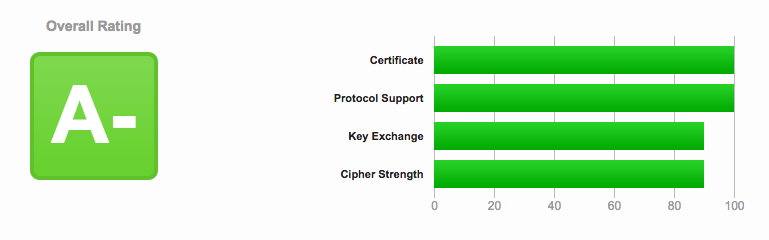
\includegraphics[width=\textwidth, scale=0.5]{validcrt1} \\ \\
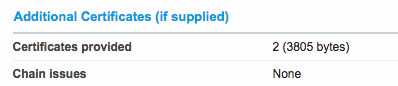
\includegraphics[width=\textwidth, scale=0.5]{validcrt2} \\ \\
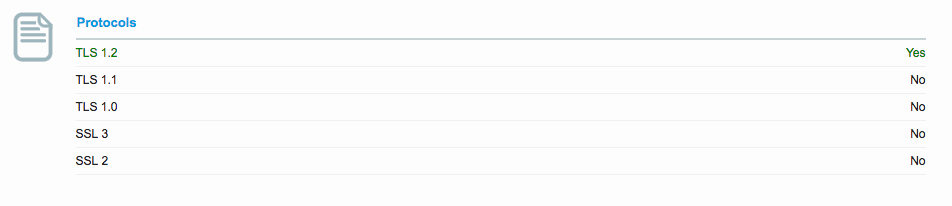
\includegraphics[width=\textwidth, scale=0.5]{validcrt3} \\ \\ \cite{check}


\section{Web Server Security}
\begin{enumerate}
\item Folder access rules. We can define different rules for every dir.
\begin{verbatim}
    <Directory /var/www>
    ...
    Order deny,allow # show order for commands. In this, Deny than allow. All are allowed by default.
    Allow from all # will allow to enter for all
    Deny from all # will deny for all
    Allow/Deny from 188.130.155.41 # Allows from that address
    ...
    </Directory>
\end{verbatim}

\item Folder access rules. We can define different rules for every dir.
\begin{verbatim}
    <Directory /var/www>
    ...
    Order deny,allow # show order for commands. In this, Deny than allow. All are allowed by default.
    Allow from all # will allow to enter for all
    Deny from all # will deny for all
    Allow/Deny from 188.130.155.41 # Allows from that address
    ...
    </Directory>
\end{verbatim}

\item IP acl. We can define them in Directory like we done above or in htaccess file, like'll do below
\item .htaccess - file rewrites access rights for directory, for easier management. Wee need add AllowOverride to Directory in webserver config.
\begin{verbatim}
    redirect /st8 https://st9.st8.os3.su #redirects from st9.os3.su/st8 to subdomain
    redirect /st10 https://st9.st10.os3.su
    ErrorDocument 404 /404.html #changes 404 error page. We also can change page for other errors
    Allow from all #Changes ACL for directory where .htaccess resides

    <Files restricted.txt> # Changes config for that files only
    order deny,allow # change order
    deny from all #make deny from all
    allow from 188.130.155.42 #let go only from our address
    </Files>

    <Files passworded.html> #Adding basic auth for that page
    AuthName "Secured zone" #Message
    AuthType Basic # Type
    AuthUserFile /var/www/.htpasswd 
    # passwod file. Can be generated with htpasswd -c /var/www/.htpasswd user

    Require valid-user #Says that require valid-user for access to that file
    </Files>
\end{verbatim}
\end{enumerate}
Trying to connect to restricted file from wrong ip \\ \\
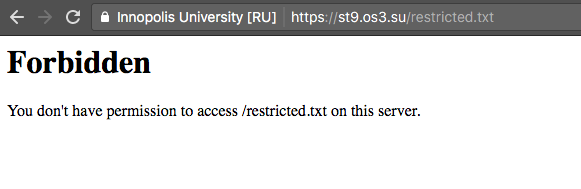
\includegraphics[width=\textwidth, scale=0.5]{forbidden} \\ \\ \\
When i try to curl from right machine \\ \\
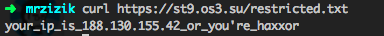
\includegraphics[width=\textwidth, scale=0.5]{restricted} \\ \\ \\
Authentication testing \\
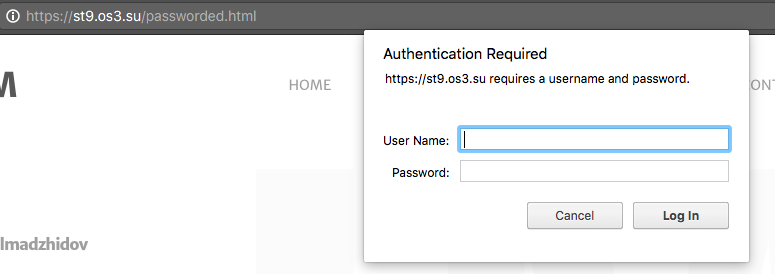
\includegraphics[width=\textwidth, scale=0.5]{auth} \\ \\

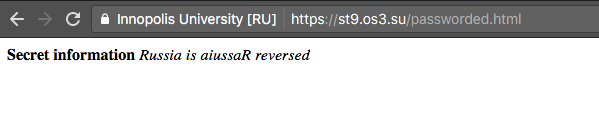
\includegraphics[width=\textwidth, scale=0.5]{auth2} \\ \\

Custom 404 error page \\ \\
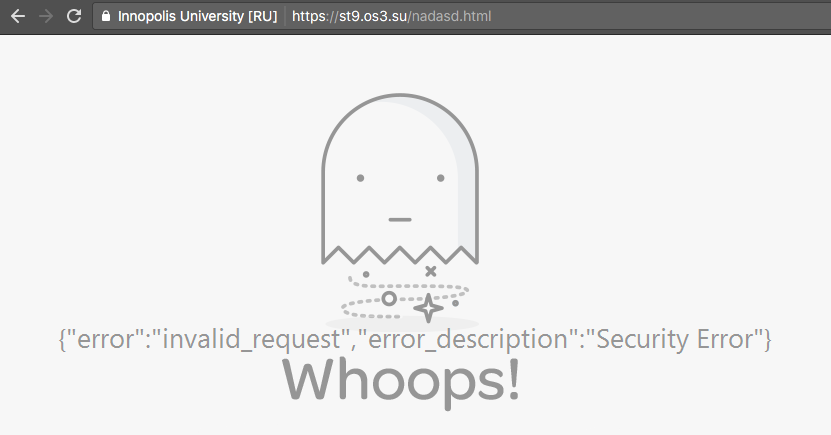
\includegraphics[width=\textwidth, scale=0.5]{404} \\ \\


\section{SSI and CGI scripts}
\begin{enumerate}
\item We need to turn on modincludes and modcgi in config and add new optionsFollowSymLinks ExecCGI
    \begin{verbatim}
        LoadModule include_module modules/mod_include.so
        LoadModule cgid_module modules/mod_cgid.so
        ...
        Options ... Includes ExecCGI
    \end{verbatim}
\item Then we need to configure .htaccess for our scripts
\begin{verbatim}
    ...
    XBitHack on #This will exec only SSI with execute bit on (chmod +x)
    AddHandler cgi-script .py # handler for python scripts
    ...
\end{verbatim}
\item Then we create our scripts
test.py
\begin{verbatim}
#!/usr/bin/env python3

print("Content-Type: text/html") #Need headers or apache wouldn't execute
print()
print ("""
    <TITLE>CGI script ! Python</TITLE>
    <H1>This is my first CGI script</H1>
    Hello, world!
"""
)
\end{verbatim}
\begin{verbatim}
<!--#echo var="DATE_LOCAL" -->
\end{verbatim}
\end{enumerate}
SSI script \\ \\
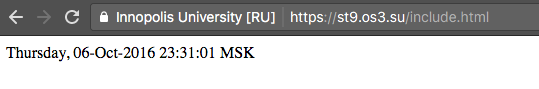
\includegraphics[width=\textwidth, scale=0.5]{ssi}\\ \\

Python script \\ \\
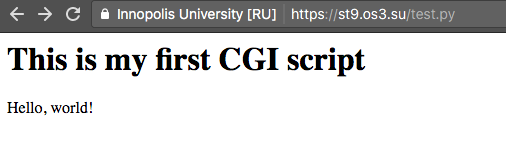
\includegraphics[width=\textwidth, scale=0.5]{cgi}\\ \\

\begin{thebibliography}{9}
\bibitem{redhat}
https://news.netcraft.com/archives/2014/02/07/are-there-really-lots-of-vulnerable-apache-web-servers.html
\bibitem{check}
https://www.ssllabs.com/ssltest/analyze.html
\end{thebibliography}
\end{document}